\begin{figure}
  \centering

  \begin{subfigure}{\ablationfigwidth}
    \centering
    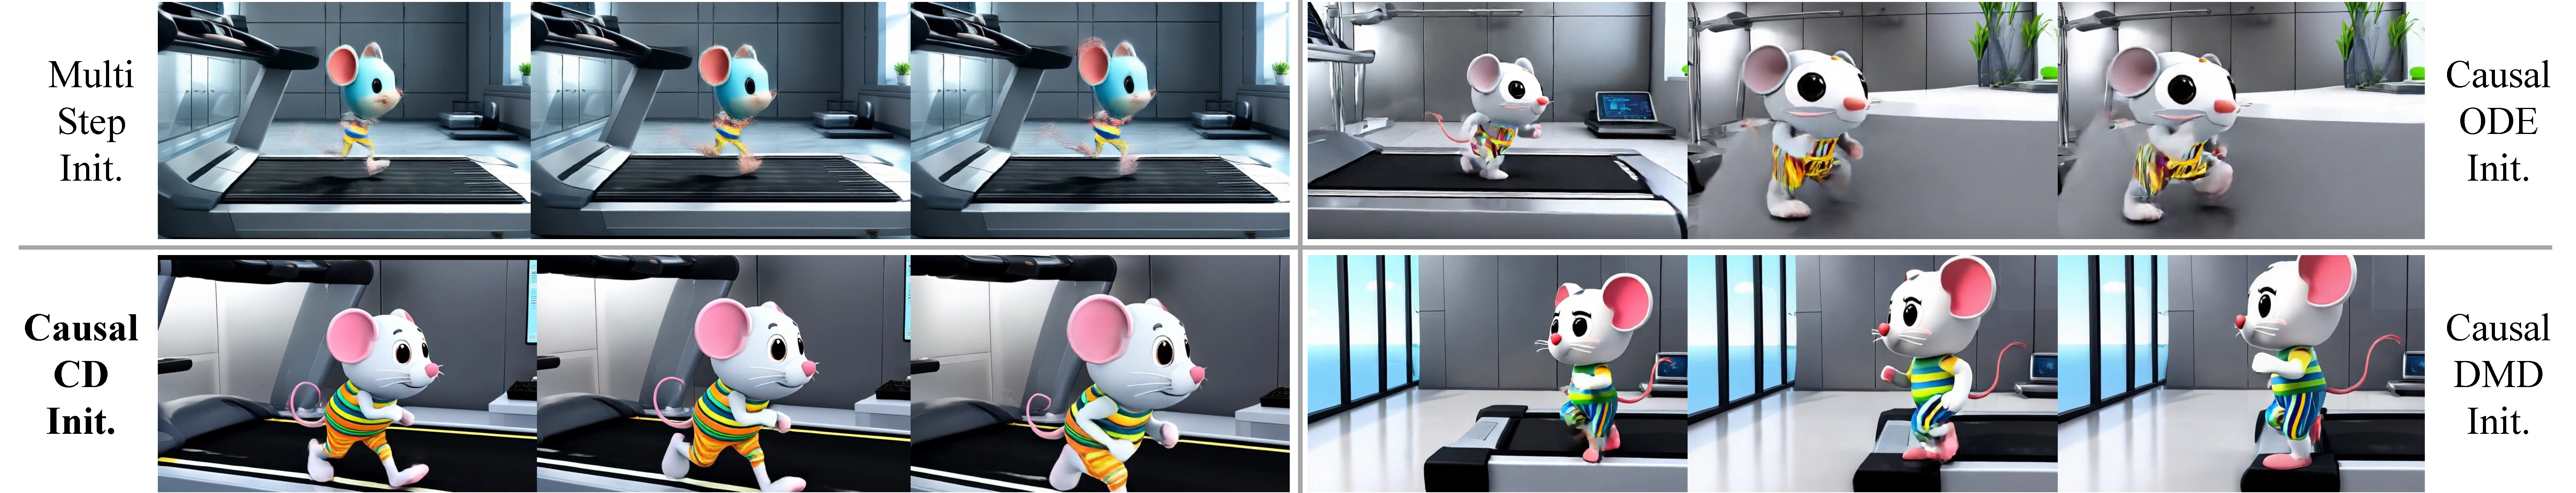
\includegraphics[width=\linewidth]{Figures/ablation_step1.pdf}
    \caption{\footnotesize \textbf{Final results of 1-step asymmetric DMD under different initializations.} AR diffusion initialization results in severe blur and almost no motion, causal ODE suffers from scene collapse, and causal DMD blurs the mouse’s legs into a single indistinguishable mass. In contrast, causal CD initialization preserves both strong dynamics and high visual quality.  Init. denotes initialization.}
  \end{subfigure}

  \vspace{0.5em}

  \begin{subfigure}{\ablationfigwidth}
    \centering
    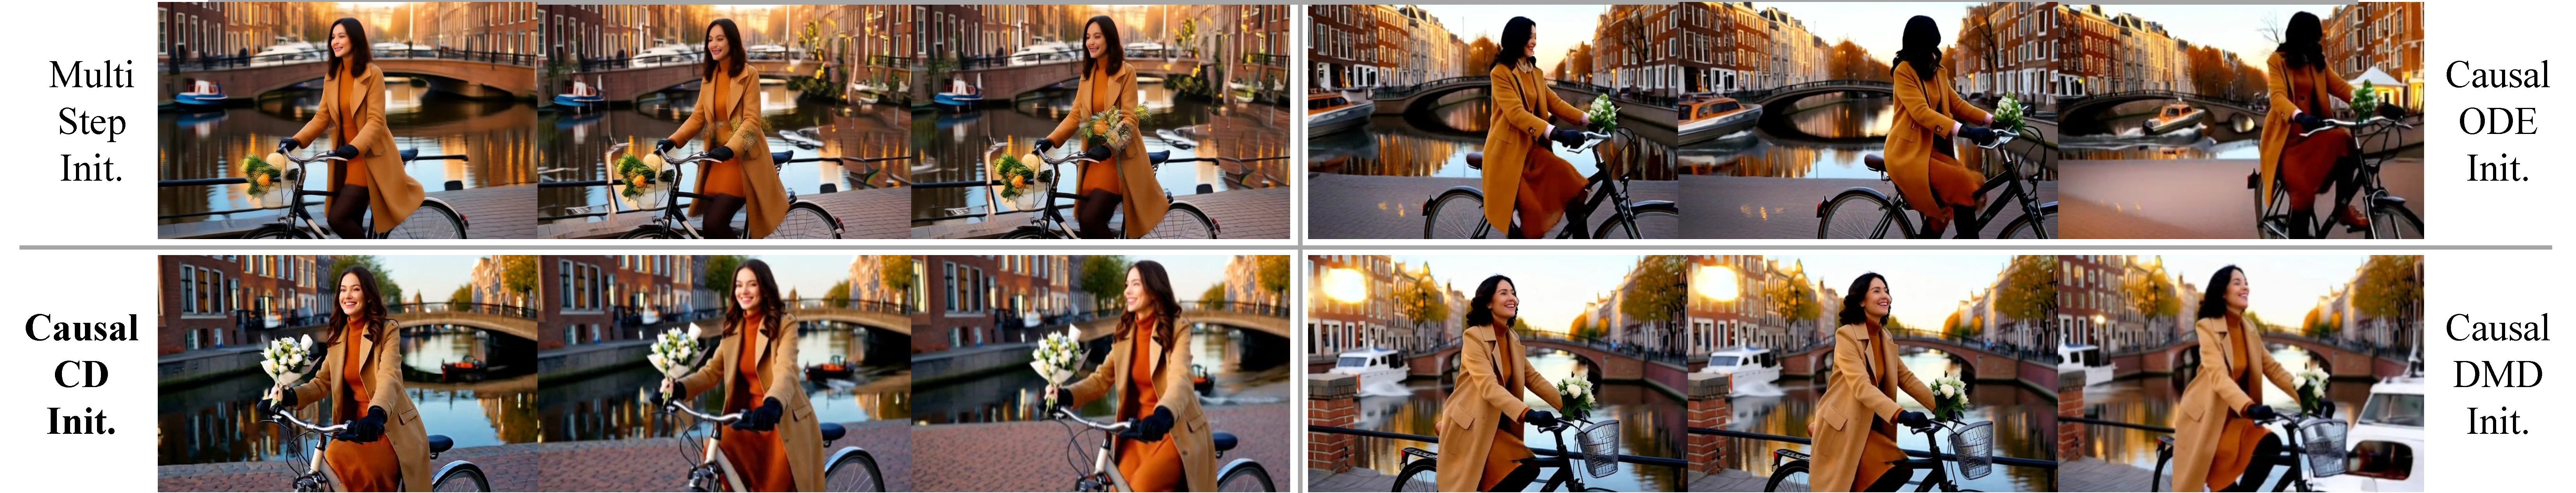
\includegraphics[width=\linewidth]{Figures/ablation_step2.pdf}
    \caption{\footnotesize \textbf{Final results of 2-step asymmetric DMD under different initializations.} Multi-step init. blurs the bouquet, causal ODE init. turns the person’s head black, and causal DMD init. introduces a bright spot in the first frame and a boat in later frames. In contrast, causal CD init. maintains stable quality. Init. denotes initialization.}
  \end{subfigure}

  \vspace{0.5em}

  \begin{subfigure}{\ablationfigwidth}
    \centering
    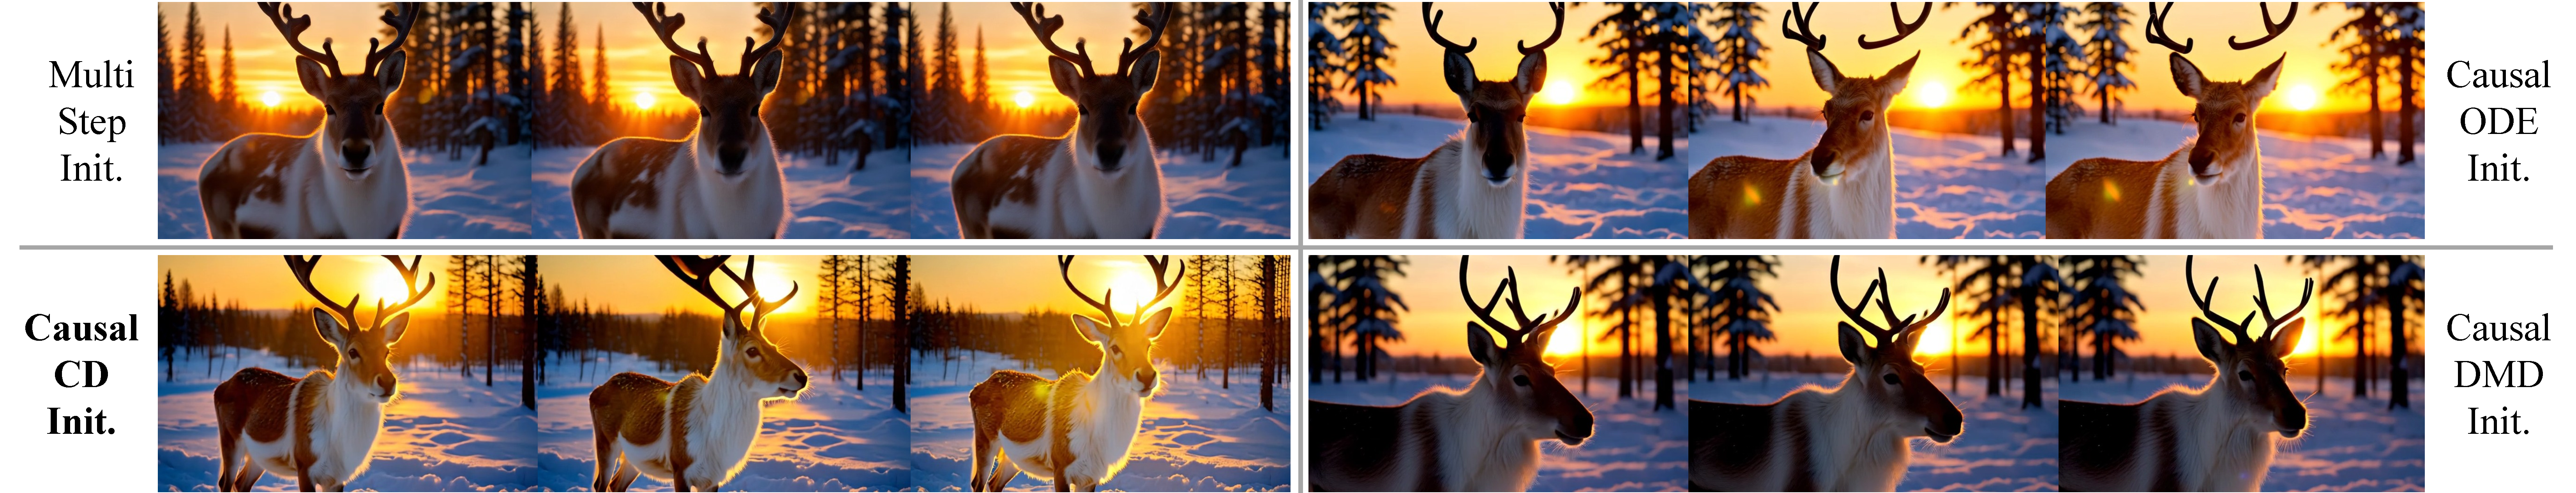
\includegraphics[width=\linewidth]{Figures/ablation_step4.pdf}
    \caption{\footnotesize \textbf{Final results of 4-step asymmetric DMD under different initializations.} Both multi-step and causal DMD initializations produce poor visual quality. Causal ODE exhibits antler separation artifacts, whereas causal CD initialization yields high-quality results. Init. denotes initialization.}
  \end{subfigure}

  \caption{\textbf{Visual comparisons after asymmetric DMD with different initializations.} Causal CD achieves results comparable to or even better than, causal ODE, whereas multi-step and causal DMD initializations perform worse.}
  \label{fig:ablation}

\end{figure}